% Template for IGARSS-2018 paper; to be used with:
%          spconf.sty  - LaTeX style file, and
%          IEEEbib.bst - IEEE bibliography style file.
% --------------------------------------------------------------------------
\documentclass{article}
\usepackage{spconf,amsmath,epsfig,graphicx}
\usepackage{subcaption}
\usepackage[noend]{algpseudocode}
\usepackage{algorithm}
\usepackage{caption}
\usepackage{url}


% Example definitions.
% --------------------
\def\x{{\mathbf x}}
\def\L{{\cal L}}

% Title.
% ------
\title{Extracting high-volume traffic routes from AIS spatial distribution maps.}
%
% Single address.
% ---------------
\name{T.L. Grobler$^{\dagger}$ and W. Kleynhans$^{\star}$$^{\ddagger}$}
\address{$\dagger$Department of Mathematical Sciences, Computer Science Division, Stellenbosch University,\\ Private Bag X1, 7602 Matieland, South Africa\\
$\star$Department
of Electrical, Electronic and Computer Engineering
University of Pretoria,\\ Pretoria 0002, South Africa\\
$\ddagger$ IMIS Global Limited, Fareham, UK}
%
% For example:
% ------------
%\address{School\\
%	Department\\
%	Address}
%
% Two addresses (uncomment and modify for two-address case).
% ----------------------------------------------------------
%\twoauthors
%  {A. Author-one, B. Author-two\sthanks{Thanks to XYZ agency for funding.}}
%	{School A-B\\
%	Department A-B\\
%	Address A-B}
%  {C. Author-three, D. Author-four\sthanks{The fourth author performed the work
%	while at ...}}
%	{School C-D\\
%	Department C-D\\
%	Address C-D}
%
\begin{document}
%\ninept
%
\maketitle
%
\begin{abstract}
In this paper we present a top-down algorithm which is capable of extracting high volume traffic routes from spatial distribution Automatic Identification System (AIS) maps (i.e. heat-maps).
We tested our algorithm on real AIS data received from vessels that were located in the Aegean sea (during January 2016). The results obtained from this test 
indicate that the proposed algorithm shows promise as it was able to detect most of the high traffic routes that a human observer would have been able to identify via a visual inspection of the same data. The ones that were not detected can be detected if we were 
to apply our algorithm in a recursive manner. We finish the paper by making suggestions on how the proposed algorithm could be improved upon.
\end{abstract}
%
\begin{keywords}
Automatic Identification System (AIS), trajectory mining, computer vision, time-series, Hough transform.
\end{keywords}

\section{Introduction}
Advances in satellite technology and communication networks have led to massive amounts of trajectory data being created. 
Trajectory data are time-stamped spatial coordinates of humans, vessels or animals and can be used to study their long-term behavioral patterns. The large increase 
in the amount of trajectory data which is now readily available necessitates the automatic processing thereof, which is the topic of this paper.
Trajectory mining refers to the process of converting recorded spatial-temporal data into usable information. Trajectory mining consist of multiple sub-parts, namely 
preprocessing, data management and pattern mining \cite{zheng2015}.

In this paper, we focus on Automatic Identification System (AIS) data. AIS is a prominent maritime vessel tracking system and is used primarily 
for collision avoidance and maritime surveillance. AIS messages, containing amongst other information the location of the vessel the message was sent from, are transmitted from transponders which are located 
on maritime vessels. Other vessels, some satellites and terrestrial shore stations are capable of receiving the transmitted AIS messages \cite{li2017}.

%The primary use case of 
%AIS is collision avoidance. Sattelites are capable of recordin g AIS signatures. To refer to the aforementioned concept the term Satelite-AIS (S-AIS) is used. The results in 
%this paper were generated by using S-AIS data.
The most basic visualization operation which one can perform with AIS data is the creation of a spatial distribution map (or simply a heat-map). A heat-map 
is created by cumulatively gridding the AIS data onto a two-dimensional grid. This map can provide 
intuitive insight into the data which can then in turn be used to improve the reduction of the original raw data using other more advanced approaches.

As we mentioned before, trajectory mining consists of different sub-blocks. The algorithm we present in this paper is a novel pattern mining approach. In contrast to many 
pattern mining approaches in literature \cite{zheng2015}, the one we present here is a top-down instead of a bottom-up approach. To clarify the previous statement, the algorithm 
takes as input an AIS heat-map and not the original raw un-gridded data-points.

The proposed algorithm works as follows. The given AIS heat-map is preprocessed using computer vision techniques. The Hough transform is then employed to extract the high volume traffic routes from the preprocessed heat-map. The extracted traffic routes are then used to segment the 
heat-map into high and low volume traffic regions.

We wish to emphasize that the approach we present in this paper is supplementary and is not intended to replace existing bottom-up approaches. It merely serves to provide additional information 
which will make it easier to process the original data via more conventional means.
The benefits of the proposed top-down method are:
\begin{itemize}
 \item As this is a top-down approach one can quickly obtain insight into the data, which can be used to better analyze the data using more conventional bottom-up approaches.
 \item High volume traffic routes used primarily for long distance travel can easily be extracted without having to do much preprocessing. 
 \item The extracted high volume traffic routes can be used to naturally segment a map into smaller regions, which in turn can be further analyzed using more conventional bottom-up approaches.
 %\item The segmented regions can be divided into low and high volume segments and in conjunction with the extracted high volume routes can be used for traffic flow analysis.
 \item In rare cases when one only has access to a trajectory heat-map this algorithm will still be able to extract useful trajectory information.
 \end{itemize}
 
 We describe the AIS dataset we made use of in Section~\ref{sec:data}. The proposed algorithm is presented in Section~\ref{sec:met}. We end the paper with some results and a conclusion.

% about the travelling patterns of humans, vehicles and animals. 
% 
% \textbf{TODO::} Moet kort literatuur opsomming gee. Insluitende wat Trajectory datamining is ens... Belangrike papers noem. Lees paar papers hier om oorsig te kry. Beskryf wat is 
% AIS data.
% 
% \textbf{TODO::} Noem dat die paper is 'n top down approach. Noem die voordele van die metode:
% a) Capable of etracting high traffic routes used primarily for long distance travel. b) Gain insight into data quickly. c) Easily subdivide data so that it can processed
% further. Have to think of more reasons as to why this top-down approach is useful. d) Identify low traffic regions and high traffic regions. e) Analyze how traffic makes 
% use of high volume routes.
% 
% \textbf{TODO::} We start with a heat-map and ask what useful information can we extract from naively gridding AIS data and analyzing the created heat-map.
% 
% Often, when we first inspect a dataset containing the temporal-spatial coordinates of multiple objects (i.e. the movements of say humans, animals or vessels)
% we would create a heat-map (grid data onto a two-dimensional grid) so that we can build some intuition (gather information) about the data.
% The information we extract from heat-maps (insight gained) can then be used to further analyze the original data. Some examples of the useful kind of information which can be extracted from a 
% heat-map include: high traffic volume routes and regions. In this paper, we present an automatic heat-map segmentation algorithm which will allow us to automatically extract the 
%  aforementioned pieces of information. In this paper we focus primarily on AIS data (shipping data). 
 
\section{Dataset}
\label{sec:data}
The dataset that was used contains one month (January 2016) of AIS messages transmitted by vessels located in European waters. This data was
obtained as part of the datAcron maritime use case (\url{http://datacron-project.eu/}) \cite{vouros2017}.  
The dataset contains messages recoded by both terrestrial as well as satellite AIS based receivers. The AIS dataset is raw and unparsed as it contains the AIS messages 
just as it was received by the AIS receivers. The dataset contains both class A and B positional reports (message types 1,2,3,18,19)
as described in the ITU-R.M 1371-5 specification. These messages contain fields such as longitude, latitude,
speed-over-ground, course-over-ground, rate of turn, navigational status, and true heading. We assumed that each vessel
can be uniquely identified by its Marine Mobile Service Identifier (MMSI). 
%\cite{itum}

\section{Methodology}
\label{sec:met}
As we mentioned in the introduction, the proposed algorithm takes as input an AIS heat-map. It also makes use of a coastline mask and a land mask. The coastline mask
marks the regions in the heat-map which are close to land and should therefore be grouped into its own unique region (segment). The land mask contains the regions of the heat-map which 
are located on land (and should therefore be excluded from the computation). During the first step of the algorithm the element-wise logarithm of the AIS heat-map, we wish to process, is taken. This visually emphasizes the high volume routes found within the heat-map. We then 
create a binary heat-map. To achieve this we first convert the heat-map (after having applied an element-wise logarithm to it) into a gray-scale intermediate heat-map. We then filter this intermediate heat-map. We make use of a median filter as it is well known for its ability to detect outliers. We then threshold (we used Otsu thresholding) the  
filtered heat-map. To clean the binary heat-map (we obtained by applying thresholding) we apply the morphological opening operator to it (which is used to remove noise from the foreground).
We then use the Hough transform to extract the lines (high volume traffic routes) from the opened binary heat-map. We then polygonize the heat-map using the extracted lines. We can then 
segment the original heat-map into different regions using the aforementioned derived polygons. The pseudo-code of the proposed segmentation algorithm is given in Algorithm 1. We discuss the most important algorithms used within the segmentation approach we 
just described in more detail in the sections that follow.  

\begin{algorithm}
 \caption{Polygon Heat-map Segmentation Algorithm}\label{euclid}
 \begin{algorithmic}[1]
 \Procedure{polySeg}{heatmap,coastlinemask,lmask}
 \State $\textrm{heatmap} \gets \log(\textrm{heat-map}+1)$
 %\Comment{emphasizes the linear tracks}
 \State $\textrm{copy} \gets \textrm{heat-map}$
 \State $\textrm{heatmap} \gets \textrm{convertToGrayscale(heatmap)}$
 %\Comment{store a copy of original}
 \State $\textrm{heatmap} \gets \textrm{maskCoastline(heatmap,coastlinemask)}$
 %\Comment{mask coastline}
 \State $\textrm{heatmap} \gets \textrm{heatmap - medianFilter(heatmap)}$ 
 %\Comment{detect outliers}
 \State $\textrm{heatmap} \gets \textrm{otsuThreshold(heatmap)}$
 %\Comment{binary segmentation}
 \State $\textrm{heat-map} \gets \textrm{binaryOpening(heat-map)}$
 %\Comment{clears the noisy region}
 \State $\textrm{lines} \gets \textrm{houghTransform(heatmap)}$
 %\Comment{extract lines from image}
 \State $\textrm{polygons} \gets \textrm{polygonize(lines,coastlinemask,lmask)}$
 %\Comment{polygonize}
 \For{polygon in polygons}
     \State $\textrm{heatmap[polygon]} \gets \textrm{average(copy[polygon])}$ 
 \EndFor
 \State $\textrm{heatmap[coastlmask]} \gets \textrm{average(copy[coastlmask])}$
 \State $\textrm{heatmap[lmask]} \gets 0$
 %\Comment{segmentation}
 \State plot(heatmap)
 
% \State $\textit{stringlen} \gets \text{length of }\textit{string}$
% \State $i \gets \textit{patlen}$
% %\BState \emph{top}:
% \If {$i > \textit{stringlen}$} \Return false
% \EndIf
% \State $j \gets \textit{patlen}$
% %\BState \emph{loop}:
% \If {$\textit{string}(i) = \textit{path}(j)$}
% \State $j \gets j-1$.
% \State $i \gets i-1$.
% \State \textbf{goto} \emph{loop}.
% \State \textbf{close};
% \EndIf
% \State $i \gets i+\max(\textit{delta}_1(\textit{string}(i)),\textit{delta}_2(j))$.
% \State \textbf{goto} \emph{top}.
 \EndProcedure
 \end{algorithmic}
 \end{algorithm}


\subsection{Otsu Thresholding}
Otsu thresholding is used to convert a gray-scale image to a binary image. Otsu's method calculates a threshold which divides 
the pixels of an image into two classes (foreground and background pixels). The pixels are divided in such a manner that the inter-class variance 
of the resulting classes are maximized \cite{otsu1979}. 

\subsection{Morphological Opening}
Morphological opening of an image is obtained by first applying the erosion operator and then applying the dilation operator to an image. 
Morphological erosion is performed by setting a pixel $(i,j)$ to the minimum of all the pixels in the neighborhood of that pixel. The size 
and shape of the neighborhood can be set arbitrarily. Dilation is a similar operator,
the only difference is that instead of using the minimun operator it uses the maximum operator. The net effect of using these two operators one after the other is that dark regions between bright features in an image are enlarged \cite{soille2013}. 

%Erosion enlarges dark regions, while shrinking bright regions.
%Dilation therefore, enlarges bright regions and shrinks dark regions.
\subsection{Hough Transform}
The Hough transform is an algorithm which can be used to detect specific shapes in a binary image. In this, paper we use it to detect lines. 
The first step in the algorithm is to compute, for every non-zero pixel, the parameters of all the lines which could pass through it. Importantly, we do these calculations using polar coordinates. 
The result of this calculation is a list of tuples associated with each pixel. Each tuple $(r,\theta)$ can be associated with a line $f$ and contains two values, 
the distance $r$ from the origin to the closest point on the line $f$ and the angle $\theta$ which is the angle formed by the line 
connecting the origin and the closest point on the line $f$ and the $x$-axis. Next we grid the list of tuples associated with each non-zero pixel onto a two-dimensional 
grid, called the accumulator, using $r$ and $\theta$ as index values. The accumulator is initialized as an all zero matrix. Every time we grid a tuple onto the accumulator 
we increment the value stored in the appropriate cell by one. If there are lines present in the image peaks will start to form in the accumulator. Next, we 
identify the peaks in the accumulator, if there are any, and use their location to compute the parameters of the possible lines contained within the image \cite{illingworth1988}. 

\subsection{Polygonization}
If we are given multiple line segments within an image we can easily segment the image into smaller polygons. The first step needed to achieve this is to determine 
all the coordinates at which the line segments intersect each other. Next we need to convert the given line 
segments into a graph $G$. The intersection points of the original line segments form the nodes of the graph $G$. The segments (these segments will be different to the original given line segments)
which connect the intersecting points will form the edges of the graph. The problem now reduces to finding the cycles in the newly formed graph $G$. This algorithm is explained in more detail in \cite{ferreira2003}.
%The Bentley–Ottmann algorithm is an efficient way to achieve this.
% \textbf{TODO::} Small description on Thresholoding. Binary opening. Houghtransform. Polygonization. Each one seperate section. Overall description of algorithm. Add picture of Hough 
% transform of the binary image and discuss. Short description of Hough transform maybe. 
 
\section{Results and Conclusion}
To test our algorithm we applied it to the AIS data described in Section~\ref{sec:data}. Note that we only used a subset of the available data as we decided to only 
consider AIS messages received from vessels located in the Aegean sea. Before we could apply our algorithm we first converted the raw pointal data described in Section~\ref{sec:data} into a heat-map.
This was achieved by gridding the data onto a two-dimensional grid. We then applied the algorithm as described in Section~\ref{sec:met} to the aforementioned heat-map. 
The original heat-map (after having taken the element-wise logarithm of it) can be found in Figure~\ref{fig7:a}. We then converted the image to gray-scale, filtered it and 
then applied the morphological opening operator to it to obtain Figure~\ref{fig7:b}. We then extracted the most obvious lines from the binary heat-map using the Hough transform. The 
extracted lines (i.e. the high volume traffic routes) is depicted in Figure~\ref{fig7:c}. We then segmented the heat-map into differing traffic regions (high and low volume) using the 
extracted lines. The result of this segmentation is depicted in Figure~\ref{fig7:d}. Closely inspecting Figure~\ref{fig7} reveals that the algorithm succeeds in extracting most of the high volume traffic routes from the heat-map.
However, not all of the routes were extracted successfully. This can be remedied by applying the algorithm in a recursive fashion, i.e. apply it again to each of the newly identified segmented regions. Moreover, 
the algorithm needs to be improved further, we are not interested in extracting the entire line as is currently done, but only in the line segments which actually correspond to high 
traffic routes. This can be accomplished by matching the extracted lines with the original heat-map and only keeping the parts of the line 
which overlays grid-cells containing many gridded AIS data-points. These improvements are to be pursued in a future endeavor.
 
In conclusion, we presented an algorithm that can extract high-traffic routes from an AIS heat-map. The extracted routes were then used to segement the image. 
Lastly, we wish to make the code for our algorithm publicly available (which in turn uses \textsc{scikit-image} \cite{scikitimage}), it can be downloaded here: \url{https://github.com/Trienko/s_analysis} .

% \textbf{TODO::} Beskryf wat reg is wat verkeerd is hoe mens iteratief kan verbeter. Goeie punt om dit regtig uit te le....
%  
% In this paper we present a heat-map segmentation algorithm. The proposed segmentation algorithm
% segments a heat-map into high traffic regions and low traffic regions. The borders of the different regions often coincide with high traffic routes. We then test the proposed 
% algorithm on a heat-map constructed from Automatic Identification System (AIS) data collected in the Celtic sea, the Channel and the Bay of Biscay. The results show that the approach shows promise and if improved further 
% it could become a viable segmentation strategy.
%  
% The first step of the algorithm is to take the elment-wise logarithm of the heat-map passed into it as an argument. This visually emphasises the high volume routes found within the heat-map. We then 
% create a binary image. To achieve this we first filter the logged heat-map. We make use of a median filter as it is well known for its ability to detect outliers. We then threshold (we used Otsu thresholding) the  
% filtered heat-map. To clean the binary heat-map (we obtained by applying thresholding) we apply the morphological opening operator to it (which is used to remove noise from the foreground).
% We then use the Hough Transform to extract the longer lines from the opened binary heat-map. We then polygonize the heat-map using the extracted lines. We can then 
% segment the original heat-map into different regions using the aforementioned derived polygons. The result of applying the above algorithm to AIS data is depicted in Figure~\ref{fig7}.
% 
% 
% Figure~\ref{fig7} highlights some of the shortcomings of this segmentation strategy. The Hough-Transform struggles to detect all 
% the lines. It especially struggles with short and closely spaced parallel lines (can be mitigated by iteratively applying the algorithm to each segmented region). It works on the assumption that straight line routes were followed (which is not guaranteed). Some of the line segments should also be removed prior to polygonization as they do not 
% represent true high volume routes. The value of the coastline segments can be separately computed within each polygon.
 
\begin{figure*}[h] 
  \begin{subfigure}[b]{0.49\linewidth}
    \centering
    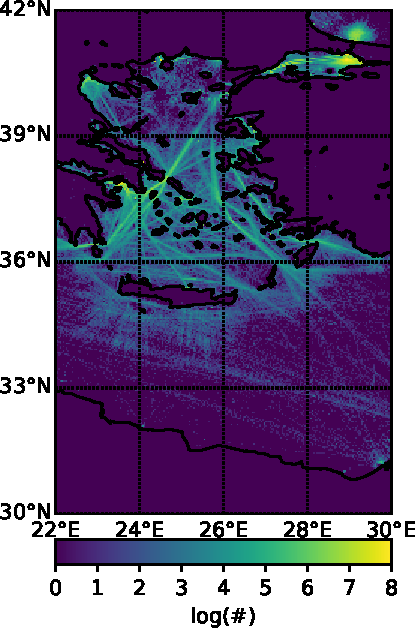
\includegraphics[width=0.7\linewidth]{AGEAN_DCRON-crop.pdf} 
    \caption{Logarithm applied} 
    \label{fig7:a} 
    \vspace{4ex}
  \end{subfigure}%% 
  \begin{subfigure}[b]{0.49\linewidth}
    \centering
    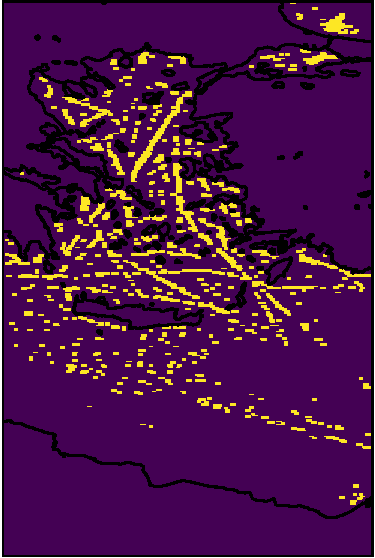
\includegraphics[width=0.59\textwidth]{AGEAN_DCRON_opened-crop.pdf} 
    \caption{Binary segmented image} 
    \label{fig7:b} 
    \vspace{13ex}
    \end{subfigure} 
  \begin{subfigure}[b]{0.49\linewidth}
    \centering
    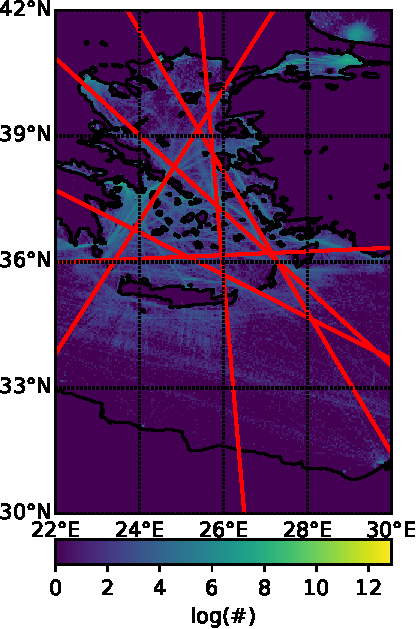
\includegraphics[width=0.7\textwidth]{AGEAN_DCRON_lines-crop.pdf} 
    \caption{Hough Transform} 
    \label{fig7:c} 
  \end{subfigure}%%
  \begin{subfigure}[b]{0.49\linewidth}
    \centering
    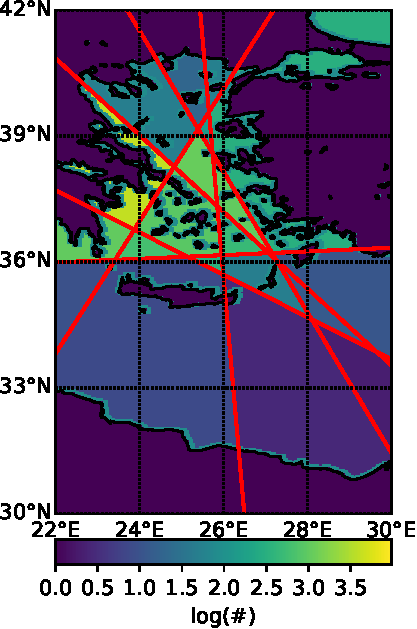
\includegraphics[width=0.7\textwidth]{AGEAN_DCRON_segmented-crop.pdf} 
    \caption{Segmented image} 
    \label{fig7:d} 
  \end{subfigure} 
  \caption{Results obtained by applying Algorithm 1 to an AIS heat-map which in turn was constructed by using AIS data received from vessels located in the Aegean sea during January 2016 [Longitude between $22^{\circ}$ and $30^{\circ}$ and Latitude between $30^{\circ}$ and $42^{\circ}$]. The top left image was obtained after the logarithm of the original input heat-map was taken (element-wise). The top right image 
  was obtained by applying binary thresholding and morphological opening to a filtered greyscale variant of the top left heat map. The right bottom heat-map depicts the lines we were able to extract 
  from the top right image using the Hough Transform. The bottom right image contains the final segmented heat map. Note that cells close to the coastline are grouped together.}
  \label{fig7} 
\end{figure*}


% \section{Introduction}
% \label{sec:intro}
% 
% These guidelines include complete descriptions of the fonts, spacing, and
% related information for producing your proceedings manuscripts. Please follow
% them and if you have any questions, direct them to Conference Management
% Services, Inc.: Phone +1-979-846-6800 or Fax +1-979-846-6900 or email
% to \verb+papers@igarss2018.org+.
% 
% \section{Formatting your paper}
% \label{sec:format}
% 
% All printed material, including text, illustrations, and charts, must be kept
% within a print area of 7 inches (178 mm) wide by 9 inches (229 mm) high. Do
% not write or print anything outside the print area. The top margin must be 1
% inch (25 mm), except for the title page, and the left margin must be 0.75 inch
% (19 mm).  All {\it text} must be in a two-column format. Columns are to be 3.39
% inches (86 mm) wide, with a 0.24 inch (6 mm) space between them. Text must be
% fully justified.
% 
% \section{PAGE TITLE SECTION}
% \label{sec:pagestyle}
% 
% The paper title (on the first page) should begin 1.38 inches (35 mm) from the
% top edge of the page, centered, completely capitalized, and in Times 14-point,
% boldface type.  The authors' name(s) and affiliation(s) appear below the title
% in capital and lower case letters.  Papers with multiple authors and
% affiliations may require two or more lines for this information.
% 
% \section{TYPE-STYLE AND FONTS}
% \label{sec:typestyle}
% 
% To achieve the best rendering in the proceedings, we
% strongly encourage you to use Times-Roman font.  In addition, this will give
% the proceedings a more uniform look.  Use a font that is no smaller than nine
% point type throughout the paper, including figure captions.
% 
% In nine point type font, capital letters are 2 mm high.  If you use the
% smallest point size, there should be no more than 3.2 lines/cm (8 lines/inch)
% vertically.  This is a minimum spacing; 2.75 lines/cm (7 lines/inch) will make
% the paper much more readable.  Larger type sizes require correspondingly larger
% vertical spacing.  Please do not double-space your paper.  True-Type 1 fonts
% are preferred.
% 
% The first paragraph in each section should not be indented, but all the
% following paragraphs within the section should be indented as these paragraphs
% demonstrate.
% 
% \section{MAJOR HEADINGS}
% \label{sec:majhead}
% 
% Major headings, for example, "1. Introduction", should appear in all capital
% letters, bold face if possible, centered in the column, with one blank line
% before, and one blank line after. Use a period (".") after the heading number,
% not a colon.
% 
% \subsection{Subheadings}
% \label{ssec:subhead}
% 
% Subheadings should appear in lower case (initial word capitalized) in
% boldface.  They should start at the left margin on a separate line.
%  
% \subsubsection{Sub-subheadings}
% \label{sssec:subsubhead}
% 
% Sub-subheadings, as in this paragraph, are discouraged. However, if you
% must use them, they should appear in lower case (initial word
% capitalized) and start at the left margin on a separate line, with paragraph
% text beginning on the following line.  They should be in italics.
% 
% \section{PRINTING YOUR PAPER}
% \label{sec:print}
% 
% Print your properly formatted text on high-quality, 8.5 x 11-inch white printer
% paper. A4 paper is also acceptable, but please leave the extra 0.5 inch (12 mm)
% empty at the BOTTOM of the page and follow the top and left margins as
% specified.  If the last page of your paper is only partially filled, arrange
% the columns so that they are evenly balanced if possible, rather than having
% one long column.
% 
% In LaTeX, to start a new column (but not a new page) and help balance the
% last-page column lengths, you can use the command ``$\backslash$pagebreak'' as
% demonstrated on this page (see the LaTeX source below).
% 
% \section{PAGE NUMBERING}
% \label{sec:page}
% 
% Please do {\bf not} paginate your paper.  Page numbers, session numbers, and
% conference identification will be inserted when the paper is included in the
% proceedings.
% 
% \section{ILLUSTRATIONS, GRAPHS, AND PHOTOGRAPHS}
% \label{sec:illust}
% 
% % \begin{figure*}
% %   \begin{minipage}[b]{.48\linewidth}
% %   \centering
% %   \centerline{\includegraphics[width=0.45\linewidth]{./FFT1.pdf}}}
% %   \vspace{1.5cm}
% %   \centerline{(b) Results 3}\medskip
% % \end{minipage}
% % \hfill
% % \begin{minipage}[b]{0.48\linewidth}
% %   \centering
% %   \centerline{\includegraphics[width=0.45\linewidth]{./FFT1.pdf}}}
% %   \vspace{1.5cm}
% %   \centerline{(c) Result 4}\medskip
% % \end{minipage}
% % \end{figure*}
% 
% Illustrations must appear within the designated margins.  They may span the two
% columns.  If possible, position illustrations at the top of columns, rather
% than in the middle or at the bottom.  Caption and number every illustration.
% All illustrations should be clear wwhen printed on a black-only printer. Color
% may be used.
% 
% Since there are many ways, often incompatible, of including images (e.g., with
% experimental results) in a LaTeX document, below is an example of how to do
% this \cite{Lamp86}.
% 
% % Below is an example of how to insert images. Delete the ``\vspace'' line,
% % uncomment the preceding line ``\centerline...'' and replace ``imageX.ps''
% % with a suitable PostScript file name.
% % -------------------------------------------------------------------------
% 
% 
% % To start a new column (but not a new page) and help balance the last-page
% % column length use \vfill\pagebreak.
% % -------------------------------------------------------------------------
% %\vfill
% %\pagebreak
% 
% 
% \section{FOOTNOTES}
% \label{sec:foot}
% 
% Use footnotes sparingly (or not at all!) and place them at the bottom of the
% column on the page on which they are referenced. Use Times 9-point type,
% single-spaced. To help your readers, avoid using footnotes altogether and
% include necessary peripheral observations in the text (within parentheses, if
% you prefer, as in this sentence).
% 
% 
% \section{COPYRIGHT FORMS}
% \label{sec:copyright}
% 
% You must also electronically sign the IEEE copyright transfer
% form when you submit your paper. We {\bf must} have this form
% before your paper can be sent to the reviewers or published in
% the proceedings. The copyright form is provided through the IEEE
% website for electronic signature. A link is provided upon
% submission of the manuscript to enter the IEEE Electronic
% Copyright Form system.

%List and number all bibliographical references at the end of the paper.  The references can be numbered in alphabetic order or in order of appearance in the document.  When referring to them in the text, type the corresponding reference number in square brackets as shown at the end of this sentence \cite{C2}.

% References should be produced using the bibtex program from suitable
% BiBTeX files (here: strings, refs, manuals). The IEEEbib.bst bibliography
% style file from IEEE produces unsorted bibliography list.
% -------------------------------------------------------------------------
\bibliographystyle{IEEEbib}
\bibliography{refs}
 
\end{document}
